\documentclass{standalone}
\usepackage{tikz}
\usetikzlibrary{patterns, positioning}

\begin{document}
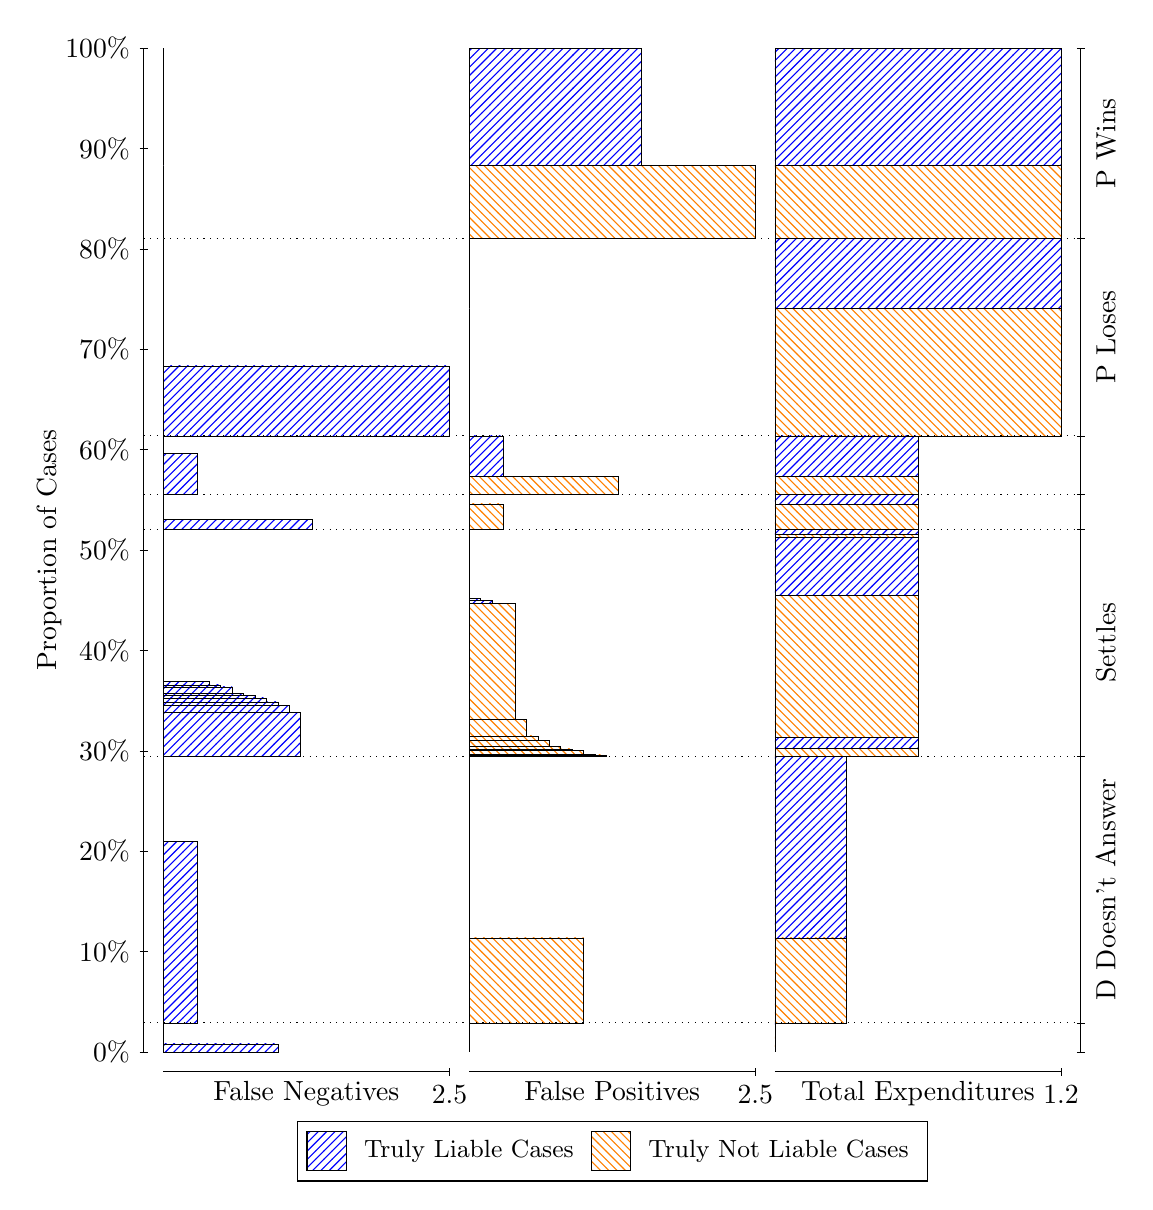
\begin{tikzpicture}
\draw[black, very thin] (1.5,1.75) -- (1.5,14.5);
\node[rotate=90, anchor=center] at (0.3, 8.125) {Proportion of Cases};
\draw[black, very thin] (1.45,1.75) -- (1.55,1.75);
\node[anchor=east] at (1.45, 1.75) {0\%};
\draw[black, very thin] (1.45,3.025) -- (1.55,3.025);
\node[anchor=east] at (1.45, 3.025) {10\%};
\draw[black, very thin] (1.45,4.3) -- (1.55,4.3);
\node[anchor=east] at (1.45, 4.3) {20\%};
\draw[black, very thin] (1.45,5.575) -- (1.55,5.575);
\node[anchor=east] at (1.45, 5.575) {30\%};
\draw[black, very thin] (1.45,6.85) -- (1.55,6.85);
\node[anchor=east] at (1.45, 6.85) {40\%};
\draw[black, very thin] (1.45,8.125) -- (1.55,8.125);
\node[anchor=east] at (1.45, 8.125) {50\%};
\draw[black, very thin] (1.45,9.4) -- (1.55,9.4);
\node[anchor=east] at (1.45, 9.4) {60\%};
\draw[black, very thin] (1.45,10.675) -- (1.55,10.675);
\node[anchor=east] at (1.45, 10.675) {70\%};
\draw[black, very thin] (1.45,11.95) -- (1.55,11.95);
\node[anchor=east] at (1.45, 11.95) {80\%};
\draw[black, very thin] (1.45,13.225) -- (1.55,13.225);
\node[anchor=east] at (1.45, 13.225) {90\%};
\draw[black, very thin] (1.45,14.5) -- (1.55,14.5);
\node[anchor=east] at (1.45, 14.5) {100\%};

\draw[black, very thin] (13.4,1.75) -- (13.4,14.5);
\draw[black, very thin] (13.35,1.75) -- (13.45,1.75);
\node[anchor=west] at (13.35, 1.75) {};
\draw[black, very thin] (13.35,2.1199) -- (13.45,2.1199);
\node[anchor=west] at (13.35, 2.1199) {};
\draw[black, very thin] (13.35,5.5074) -- (13.45,5.5074);
\node[anchor=west] at (13.35, 5.5074) {};
\draw[black, very thin] (13.35,8.3893) -- (13.45,8.3893);
\node[anchor=west] at (13.35, 8.3893) {};
\draw[black, very thin] (13.35,8.8331) -- (13.45,8.8331);
\node[anchor=west] at (13.35, 8.8331) {};
\draw[black, very thin] (13.35,9.5746) -- (13.45,9.5746);
\node[anchor=west] at (13.35, 9.5746) {};
\draw[black, very thin] (13.35,12.08) -- (13.45,12.08);
\node[anchor=west] at (13.35, 12.08) {};
\draw[black, very thin] (13.35,14.5) -- (13.45,14.5);
\node[anchor=west] at (13.35, 14.5) {};

\draw[black, very thin, pattern color=blue, pattern=north east lines] (1.75,1.75) rectangle (3.2033,1.8515);
\draw[black, very thin, pattern color=orange, pattern=north west lines] (1.75,1.8515) rectangle (1.75,2.1199);
\draw[black, very thin, pattern color=blue, pattern=north east lines] (1.75,2.1199) rectangle (2.186,4.4279);
\draw[black, very thin, pattern color=orange, pattern=north west lines] (1.75,4.4279) rectangle (1.75,5.5074);
\draw[black, very thin, pattern color=blue, pattern=north east lines] (1.75,5.5074) rectangle (3.494,6.0645);
\draw[black, very thin, pattern color=blue, pattern=north east lines] (1.75,6.0645) rectangle (3.3487,6.1551);
\draw[black, very thin, pattern color=blue, pattern=north east lines] (1.75,6.1551) rectangle (3.2033,6.196);
\draw[black, very thin, pattern color=blue, pattern=north east lines] (1.75,6.196) rectangle (3.058,6.2437);
\draw[black, very thin, pattern color=blue, pattern=north east lines] (1.75,6.2437) rectangle (3.058,6.2481);
\draw[black, very thin, pattern color=blue, pattern=north east lines] (1.75,6.2481) rectangle (2.9127,6.2823);
\draw[black, very thin, pattern color=blue, pattern=north east lines] (1.75,6.2823) rectangle (2.7673,6.3036);
\draw[black, very thin, pattern color=blue, pattern=north east lines] (1.75,6.3036) rectangle (2.622,6.3866);
\draw[black, very thin, pattern color=blue, pattern=north east lines] (1.75,6.3866) rectangle (2.4767,6.4111);
\draw[black, very thin, pattern color=blue, pattern=north east lines] (1.75,6.4111) rectangle (2.3313,6.4535);
\draw[black, very thin, pattern color=orange, pattern=north west lines] (1.75,6.4535) rectangle (1.75,8.3893);
\draw[black, very thin, pattern color=blue, pattern=north east lines] (1.75,8.3893) rectangle (3.6393,8.5118);
\draw[black, very thin, pattern color=orange, pattern=north west lines] (1.75,8.5118) rectangle (1.75,8.8331);
\draw[black, very thin, pattern color=blue, pattern=north east lines] (1.75,8.8331) rectangle (2.186,9.3512);
\draw[black, very thin, pattern color=orange, pattern=north west lines] (1.75,9.3512) rectangle (1.75,9.5746);
\draw[black, very thin, pattern color=blue, pattern=north east lines] (1.75,9.5746) rectangle (5.3833,10.462);
\draw[black, very thin, pattern color=orange, pattern=north west lines] (1.75,10.462) rectangle (1.75,12.08);
\draw[black, very thin, pattern color=orange, pattern=north west lines] (1.75,12.08) rectangle (1.75,13.008);
\draw[black, very thin, pattern color=blue, pattern=north east lines] (1.75,13.008) rectangle (1.75,14.5);
\draw[black, very thin, pattern color=orange, pattern=north west lines] (5.6333,1.75) rectangle (5.6333,2.0184);
\draw[black, very thin, pattern color=blue, pattern=north east lines] (5.6333,2.0184) rectangle (5.6333,2.1199);
\draw[black, very thin, pattern color=orange, pattern=north west lines] (5.6333,2.1199) rectangle (7.0867,3.1994);
\draw[black, very thin, pattern color=blue, pattern=north east lines] (5.6333,3.1994) rectangle (5.6333,5.5074);
\draw[black, very thin, pattern color=orange, pattern=north west lines] (5.6333,5.5074) rectangle (7.3773,5.5219);
\draw[black, very thin, pattern color=orange, pattern=north west lines] (5.6333,5.5219) rectangle (7.232,5.5322);
\draw[black, very thin, pattern color=orange, pattern=north west lines] (5.6333,5.5322) rectangle (7.0867,5.5833);
\draw[black, very thin, pattern color=orange, pattern=north west lines] (5.6333,5.5833) rectangle (6.9413,5.5987);
\draw[black, very thin, pattern color=orange, pattern=north west lines] (5.6333,5.5987) rectangle (6.796,5.6309);
\draw[black, very thin, pattern color=orange, pattern=north west lines] (5.6333,5.6309) rectangle (6.6507,5.7042);
\draw[black, very thin, pattern color=orange, pattern=north west lines] (5.6333,5.7042) rectangle (6.5053,5.7645);
\draw[black, very thin, pattern color=orange, pattern=north west lines] (5.6333,5.7645) rectangle (6.36,5.9762);
\draw[black, very thin, pattern color=orange, pattern=north west lines] (5.6333,5.9762) rectangle (6.2147,7.4431);
\draw[black, very thin, pattern color=blue, pattern=north east lines] (5.6333,7.4431) rectangle (5.924,7.4856);
\draw[black, very thin, pattern color=blue, pattern=north east lines] (5.6333,7.4856) rectangle (5.7787,7.51);
\draw[black, very thin, pattern color=blue, pattern=north east lines] (5.6333,7.51) rectangle (5.6333,8.3893);
\draw[black, very thin, pattern color=orange, pattern=north west lines] (5.6333,8.3893) rectangle (6.0693,8.7106);
\draw[black, very thin, pattern color=blue, pattern=north east lines] (5.6333,8.7106) rectangle (5.6333,8.8331);
\draw[black, very thin, pattern color=orange, pattern=north west lines] (5.6333,8.8331) rectangle (7.5227,9.0566);
\draw[black, very thin, pattern color=blue, pattern=north east lines] (5.6333,9.0566) rectangle (6.0693,9.5746);
\draw[black, very thin, pattern color=orange, pattern=north west lines] (5.6333,9.5746) rectangle (5.6333,11.193);
\draw[black, very thin, pattern color=blue, pattern=north east lines] (5.6333,11.193) rectangle (5.6333,12.08);
\draw[black, very thin, pattern color=orange, pattern=north west lines] (5.6333,12.08) rectangle (9.2667,13.008);
\draw[black, very thin, pattern color=blue, pattern=north east lines] (5.6333,13.008) rectangle (7.8133,14.5);
\draw[black, very thin, pattern color=orange, pattern=north west lines] (9.5167,1.75) rectangle (9.5167,2.0184);
\draw[black, very thin, pattern color=blue, pattern=north east lines] (9.5167,2.0184) rectangle (9.5167,2.1199);
\draw[black, very thin, pattern color=orange, pattern=north west lines] (9.5167,2.1199) rectangle (10.425,3.1994);
\draw[black, very thin, pattern color=blue, pattern=north east lines] (9.5167,3.1994) rectangle (10.425,5.5074);
\draw[black, very thin, pattern color=orange, pattern=north west lines] (9.5167,5.5074) rectangle (11.333,5.601);
\draw[black, very thin, pattern color=blue, pattern=north east lines] (9.5167,5.601) rectangle (11.333,5.7426);
\draw[black, very thin, pattern color=orange, pattern=north west lines] (9.5167,5.7426) rectangle (11.333,7.5519);
\draw[black, very thin, pattern color=blue, pattern=north east lines] (9.5167,7.5519) rectangle (11.333,8.2883);
\draw[black, very thin, pattern color=orange, pattern=north west lines] (9.5167,8.2883) rectangle (11.333,8.321);
\draw[black, very thin, pattern color=blue, pattern=north east lines] (9.5167,8.321) rectangle (11.333,8.3893);
\draw[black, very thin, pattern color=orange, pattern=north west lines] (9.5167,8.3893) rectangle (11.333,8.7106);
\draw[black, very thin, pattern color=blue, pattern=north east lines] (9.5167,8.7106) rectangle (11.333,8.8331);
\draw[black, very thin, pattern color=orange, pattern=north west lines] (9.5167,8.8331) rectangle (11.333,9.0566);
\draw[black, very thin, pattern color=blue, pattern=north east lines] (9.5167,9.0566) rectangle (11.333,9.5746);
\draw[black, very thin, pattern color=orange, pattern=north west lines] (9.5167,9.5746) rectangle (13.15,11.193);
\draw[black, very thin, pattern color=blue, pattern=north east lines] (9.5167,11.193) rectangle (13.15,12.08);
\draw[black, very thin, pattern color=orange, pattern=north west lines] (9.5167,12.08) rectangle (13.15,13.008);
\draw[black, very thin, pattern color=blue, pattern=north east lines] (9.5167,13.008) rectangle (13.15,14.5);
\draw[black, dotted] (1.5,2.1199) -- (13.4,2.1199);
\draw[black, dotted] (1.5,5.5074) -- (13.4,5.5074);
\draw[black, dotted] (1.5,8.3893) -- (13.4,8.3893);
\draw[black, dotted] (1.5,8.8331) -- (13.4,8.8331);
\draw[black, dotted] (1.5,9.5746) -- (13.4,9.5746);
\draw[black, dotted] (1.5,12.08) -- (13.4,12.08);
\draw[black, very thin] (1.75,1.5) -- (5.3833,1.5);
\node[anchor=north] at (3.5667, 1.5) {False Negatives};
\draw[black, very thin] (5.3833,1.45) -- (5.3833,1.55);
\node[anchor=north] at (5.3833, 1.45) {2.5};

\draw[black, very thin] (5.6333,1.5) -- (9.2667,1.5);
\node[anchor=north] at (7.45, 1.5) {False Positives};
\draw[black, very thin] (9.2667,1.45) -- (9.2667,1.55);
\node[anchor=north] at (9.2667, 1.45) {2.5};

\draw[black, very thin] (9.5167,1.5) -- (13.15,1.5);
\node[anchor=north] at (11.333, 1.5) {Total Expenditures};
\draw[black, very thin] (13.15,1.45) -- (13.15,1.55);
\node[anchor=north] at (13.15, 1.45) {1.2};


\node[black, centered, rotate=90] at (13.72, 3.8137) {D Doesn't Answer};
\node[black, centered, rotate=90] at (13.72, 6.9483) {Settles};


\node[black, centered, rotate=90] at (13.72, 10.827) {P Loses};
\node[black, centered, rotate=90] at (13.72, 13.29) {P Wins};

\draw (7.449999999999999,1.5) node[draw=none] (baseCoordinate) {};
\begin{scope}[align=center]
        \matrix[scale=0.5, draw=black, below=0.5cm of baseCoordinate, nodes={draw}, column sep=0.1cm]{
            \node[rectangle, draw, minimum width=0.5cm, minimum height=0.5cm, pattern=north east lines, pattern color=blue] {}; &
            \node[draw=none, font=\small] (B) {Truly Liable Cases}; &
            \node[rectangle, draw, minimum width=0.5cm, minimum height=0.5cm, pattern=north west lines, pattern color=orange] {}; &
            \node[draw=none, font=\small] (B) {Truly Not Liable Cases}; \\
            };
\end{scope}

\end{tikzpicture}
\end{document}